\newcommand{\spywareTagResultsAucTable}{
    \begin{table}[H]
        \centering
        \begin{tabular}{|p{2,8cm}||p{2,8cm} p{2,8cm} p{2,8cm}|}
            \hline
            Spyware Tag & ALOHA & Joint Embedding & Proposed Model \\
            \hline
            AUC-ROC & 0.960$\pm$0.002 & 0.966$\pm$0.005 & \textBF{0.974$\pm$0.002} \\
            \hline
        \end{tabular}
        \caption{AUC-ROC (Area Under Curve) of the different models for the \textbf{Spyware Tag} prediction task. Results were aggregated over \textBF{3} training runs with different weight initializations and minibatch orderings. Best results are shown in \textbf{bold}.} \label{tab:spywareTag_auc}
    \end{table}
}

\newcommand{\spywareTagResultsAtFprTable}{
    \begin{center}
        \begin{longtable}[c]{|p{3,2cm}||p{1,8cm} p{1,8cm} p{1,8cm} p{1,8cm} p{1,8cm}|}
            \hline
            Spyware Tag & \multicolumn{5}{c|}{{FPR}} \\
            & $10^{-5}$ & $10^{-4}$ & $10^{-3}$ & $10^{-2}$ & $10^{-1}$ \\
            \hline
            \endfirsthead

            \caption*{\raggedright ...continued from previous page} \\
            \hline
            Spyware Tag & \multicolumn{5}{c|}{\textbf{FPR}} \\
            & $10^{-5}$ & $10^{-4}$ & $10^{-3}$ & $10^{-2}$ & $10^{-1}$ \\
            \hline
            \endhead

            \caption*{\raggedleft ...continued on next page} \\
            \endfoot

            \caption{Mean and standard deviation results (TPR, Accuracy, Recall, Precision and F1-Score) of the different models for the \textbf{Spyware Tag} prediction task at different \textbf{FPR}s (\textit{False Positive Rates}). Results were aggregated over \textBF{3} training runs with different weight initializations and minibatch orderings. Best results are shown in \textbf{bold}. Under \textbf{TPR} results are also presented the percentage reduction in mean detection error and in ROC curve standard deviation introduced by the \textit{Proposed Model} with respect to both \textit{ALOHA} model and \textit{Joint Embedding}.} \label{tab:spywareTag_results_at_fpr} \\
            \endlastfoot

            \multicolumn{6}{|c|}{\textbf{TPR}} \\
            \hline
            ALOHA & 0.086$\pm$0.058 & 0.097$\pm$0.049 & 0.098$\pm$0.049 & 0.604$\pm$0.007 & 0.884$\pm$0.014 \\
            Joint Embedding & \textBF{0.120$\pm$0.015} & 0.312$\pm$0.009 & \textBF{0.359$\pm$0.065} & 0.643$\pm$0.032 & 0.896$\pm$0.021 \\
            Proposed Model & 0.107$\pm$0.095 & \textBF{0.324$\pm$0.011} & 0.333$\pm$0.002 & \textBF{0.649$\pm$0.026} & \textBF{0.939$\pm$0.013} \\
            \hline
            Error Reduction wrt \newline ALOHA & 2.3\% & 25.1\% & 26.1\% & 11.4\% & 47.4\% \\
            Error Reduction wrt \newline Joint Embedding & -1.5\% & 1.7\% & -4.1\% & 1.7\% & 41.3\% \\
            \hline
            Std Reduction wrt \newline ALOHA & -63.8\% & 77.6\% & 95.9\% & -271.4\% & 7.1\% \\
            Std Reduction wrt \newline Joint Embedding & -533.3\% & -22.2\% & 96.9\% & 18.8\% & 38.1\% \\
            \hline
            \multicolumn{6}{|c|}{\textbf{Accuracy}} \\
            \hline
            ALOHA & 0.902$\pm$0.006 & 0.903$\pm$0.005 & 0.903$\pm$0.005 & 0.949$\pm$0.001 & 0.898$\pm$0.001 \\
            Joint Embedding & \textBF{0.906$\pm$0.002} & 0.926$\pm$0.001 & \textBF{0.931$\pm$0.007} & 0.953$\pm$0.003 & 0.900$\pm$0.002 \\
            Proposed Model & 0.905$\pm$0.010 & \textBF{0.928$\pm$0.001} & 0.928$\pm$0.000 & \textBF{0.954$\pm$0.003} & \textBF{0.904$\pm$0.001} \\
            \hline
            \multicolumn{6}{|c|}{\textbf{Recall}} \\
            \hline
            ALOHA & 0.086$\pm$0.058 & 0.097$\pm$0.049 & 0.098$\pm$0.049 & 0.604$\pm$0.007 & 0.884$\pm$0.014 \\
            Joint Embedding & \textBF{0.120$\pm$0.015} & 0.312$\pm$0.009 & \textBF{0.359$\pm$0.065} & 0.643$\pm$0.032 & 0.896$\pm$0.021 \\
            Proposed Model & 0.107$\pm$0.095 & \textBF{0.324$\pm$0.011} & 0.333$\pm$0.002 & \textBF{0.649$\pm$0.026} & \textBF{0.939$\pm$0.013} \\
            \hline
            \multicolumn{6}{|c|}{\textbf{Precision}} \\
            \hline
            ALOHA & 0.999$\pm$0.001 & 0.992$\pm$0.004 & 0.908$\pm$0.033 & 0.878$\pm$0.001 & 0.514$\pm$0.004 \\
            Joint Embedding & \textBF{0.999$\pm$0.000} & \textBF{0.997$\pm$0.000} & \textBF{0.977$\pm$0.004} & 0.885$\pm$0.005 & 0.517$\pm$0.006 \\
            Proposed Model & 0.999$\pm$0.001 & \textBF{0.997$\pm$0.000} & 0.976$\pm$0.000 & \textBF{0.886$\pm$0.004} & \textBF{0.529$\pm$0.003} \\
            \hline
            \multicolumn{6}{|c|}{\textbf{F1 Score}} \\
            \hline
            ALOHA & 0.152$\pm$0.097 & 0.173$\pm$0.079 & 0.174$\pm$0.079 & 0.716$\pm$0.005 & 0.650$\pm$0.007 \\
            Joint Embedding & \textBF{0.214$\pm$0.024} & 0.475$\pm$0.011 & \textBF{0.522$\pm$0.068} & 0.745$\pm$0.023 & 0.656$\pm$0.010 \\
            Proposed Model & 0.180$\pm$0.150 & \textBF{0.488$\pm$0.012} & 0.497$\pm$0.002 & \textBF{0.749$\pm$0.019} & \textBF{0.677$\pm$0.006} \\
            \hline
        \end{longtable}
    \end{center}
}

\newcommand{\spywareTagResultsSummaryTable}{
    \begin{table}[H]
        \centering
        \begin{tabular}{|p{3,2cm}||p{1,8cm} p{1,8cm} p{1,8cm} p{1,8cm} p{1,8cm}|}
            \hline
            \multicolumn{6}{|c|}{Spyware Tag (at FPR $=1\%$)} \\
            \hline
            Model & TPR & Accuracy & Precision & Recall & F1 score \\
            \hline
            ALOHA & 0.604$\pm$0.007 & 0.949$\pm$0.001 & 0.878$\pm$0.001 & 0.604$\pm$0.007 & 0.716$\pm$0.005 \\
            Joint Embedding & 0.643$\pm$0.032 & 0.953$\pm$0.003 & 0.885$\pm$0.005 & 0.643$\pm$0.032 & 0.745$\pm$0.023 \\
            Proposed Model & \textBF{0.649$\pm$0.026} & \textBF{0.954$\pm$0.003} & \textBF{0.886$\pm$0.004} & \textBF{0.649$\pm$0.026} & \textBF{0.749$\pm$0.019} \\
            \hline
        \end{tabular}
        \caption{Summary of the mean and standard deviation results of the different models for the \textbf{Spyware Tag} prediction task at \textbf{FPR} $=1\%$. Results were aggregated over \textBF{3} training runs with different weight initializations and minibatch orderings. Best results are shown in \textbf{bold}.} \label{tab:spywareTag_result_summary}
    \end{table}
}

\newcommand{\spywareTagRocAloha}{
    \begin{figure}[H]
        \vspace*{-0.5cm}
        \centering
        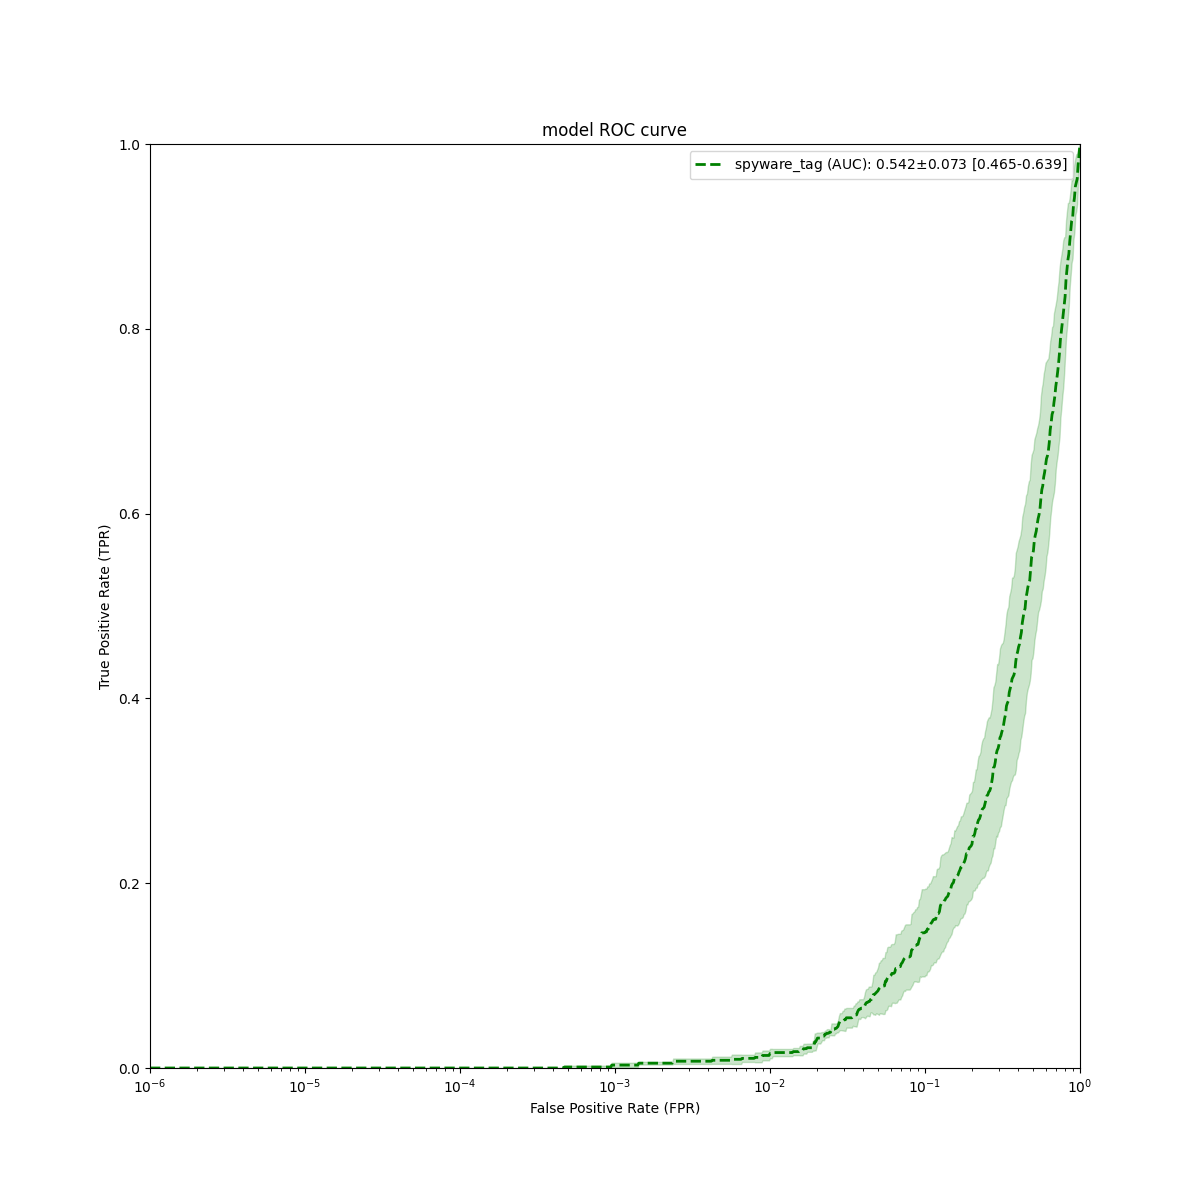
\includegraphics[width=0.6\textwidth]{./results/spyware_tag_roc_aloha.png}
        \vspace*{-0.2cm}
        \caption{ROC curve and AUC statistics of \textBF{ALOHA} model for the \textbf{Spyware Tag}. The line represents the \textit{mean} TPR at a given FPR, while the shaded region represents the \textit{standard deviation}. Statistics were computed over \textBF{3} training runs, each with random parameter initialization.}
        \label{fig:spywareTagRocAloha}
    \end{figure}
}

\newcommand{\spywareTagRocJointEmbedding}{
    \begin{figure}[H]
        \vspace*{-0.5cm}
        \centering
        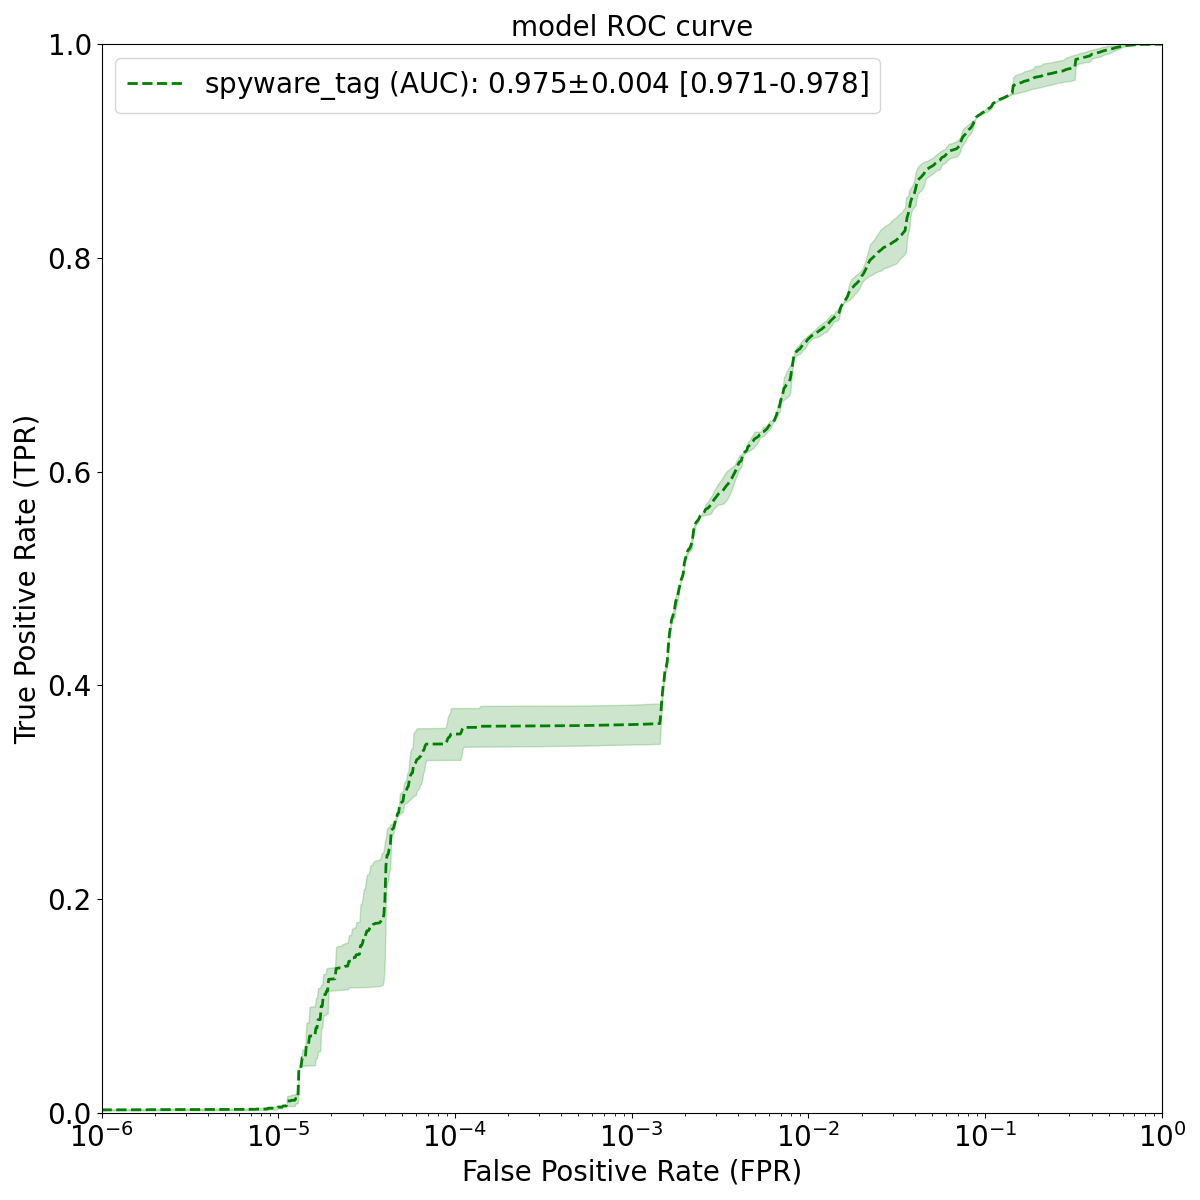
\includegraphics[width=0.6\textwidth]{./results/spyware_tag_roc_jointEmbedding.png}
        \vspace*{-0.2cm}
        \caption{ROC curve and AUC statistics of \textBF{Joint Embedding} model for the \textbf{Spyware Tag}. The line represents the \textit{mean} TPR at a given FPR, while the shaded region represents the \textit{standard deviation}. Statistics were computed over \textBF{3} training runs, each with random parameter initialization.}
        \label{fig:spywareTagRocJointEmbedding}
    \end{figure}
}

\newcommand{\spywareTagRocProposedMethod}{
    \begin{figure}[H]
        \vspace*{-0.5cm}
        \centering
        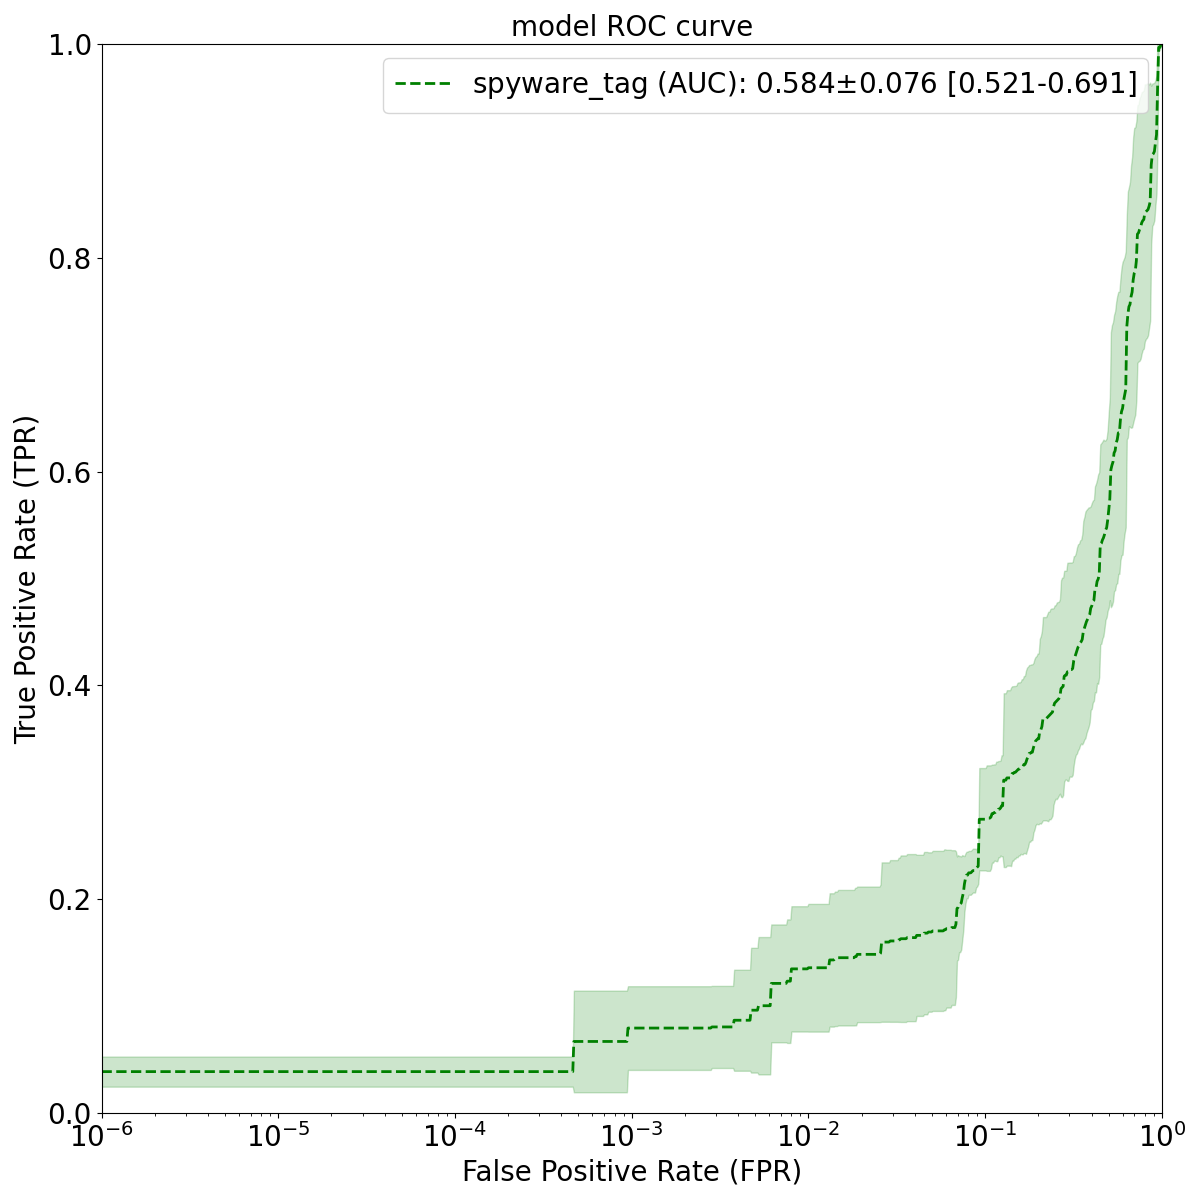
\includegraphics[width=0.6\textwidth]{./results/spyware_tag_roc_proposedModel.png}
        \vspace*{-0.2cm}
        \caption{ROC curve and AUC statistics of \textBF{Proposed Model} for the \textbf{Spyware Tag}. The line represents the \textit{mean} TPR at a given FPR, while the shaded region represents the \textit{standard deviation}. Statistics were computed over \textBF{3} training runs, each with random parameter initialization.}
        \label{fig:spywareTagRocProposedModel}
    \end{figure}
}
